% !TEX program = xelatex
\documentclass[UTF8,fontset=fandol,a4paper,11pt]{ctexart}
\usepackage[margin=21mm,top=23mm,bottom=22mm,headheight=16pt]{geometry}
\usepackage{amsmath,amssymb,mathtools,bm}
\usepackage{tikz}
\usetikzlibrary{arrows.meta,calc,angles,quotes,patterns}
\usepackage{xcolor,booktabs,array,longtable,enumitem,fancyhdr,needspace}
\usepackage[unicode,hidelinks]{hyperref}
\definecolor{ink}{HTML}{24343C}
\definecolor{accent}{HTML}{166A70}
\definecolor{muted}{HTML}{65747A}
\definecolor{rulegray}{HTML}{D4DDE0}
\definecolor{warm}{HTML}{966037}
\color{ink}
\setlength{\parindent}{2em}
\setlength{\parskip}{4pt}
\linespread{1.12}
\AtBeginDocument{\setlength{\abovedisplayskip}{6pt plus 2pt minus 1pt}
\setlength{\belowdisplayskip}{6pt plus 2pt minus 1pt}
\setlength{\abovedisplayshortskip}{0pt plus 1pt}
\setlength{\belowdisplayshortskip}{4pt plus 1pt}}
\setlist[enumerate]{label=(\arabic*),leftmargin=2.3em,itemsep=3pt,topsep=4pt}
\setlist[itemize]{leftmargin=2em,itemsep=2pt,topsep=4pt}
\allowdisplaybreaks[1]
\setlength{\emergencystretch}{2em}
\setcounter{secnumdepth}{0}
\providecommand{\tightlist}{\setlength{\itemsep}{0pt}\setlength{\parskip}{0pt}}
\ctexset{section={format=\Large\bfseries\color{accent},beforeskip=10pt,afterskip=9pt},
subsection={format=\normalsize\bfseries\color{accent},beforeskip=10pt,afterskip=4pt},
subsubsection={format=\normalsize\bfseries,beforeskip=8pt,afterskip=3pt}}
\pagestyle{fancy}
\fancyhf{}
\fancyhead[L]{\small\color{muted}物理学难题集萃}
% 页眉仅保留书名；版本名称只在封面显示。
\fancyfoot[L]{\small\color{muted}\chapterlabel}
\fancyfoot[R]{\small\thepage}
\renewcommand{\headrulewidth}{0.4pt}
\renewcommand{\footrulewidth}{0pt}
\newcommand{\dd}{\mathop{}\!\mathrm{d}}
\newcommand{\vect}[1]{\bm{#1}}
\newcommand{\tagline}[1]{\noindent{\small\color{muted}#1}\par}
\newcommand{\result}[1]{\begin{equation*}\boxed{#1}\end{equation*}}
\newcommand{\figcaption}[1]{\par\vspace{2pt}{\small\color{muted}#1}\par}
\newcommand{\teach}[2]{\Needspace{4\baselineskip}\subsection*{讲解要点与追问}#1\par\smallskip\noindent\textbf{追问：}#2\par}
\newcommand{\workarea}{\par\vspace{7mm}\noindent{\small\color{muted}作答区}\par\vspace{4mm}
\noindent\textcolor{rulegray}{\rule{\linewidth}{0.3pt}}\par\vspace{16mm}
\noindent\textcolor{rulegray}{\rule{\linewidth}{0.3pt}}\par\vspace{16mm}
\noindent\textcolor{rulegray}{\rule{\linewidth}{0.3pt}}\par\vspace{16mm}
\noindent\textcolor{rulegray}{\rule{\linewidth}{0.3pt}}}
\tikzset{axis/.style={-{Stealth[length=2mm]},thin,color=muted},
motion/.style={-{Stealth[length=2.3mm]},thick,color=accent},
force/.style={-{Stealth[length=2.3mm]},thick,color=warm},
traj/.style={thick,color=accent},guide/.style={dashed,thin,color=muted},
object/.style={thick,color=ink},every node/.style={font=\small}}\widowpenalty=10000\clubpenalty=10000\displaywidowpenalty=10000\newcommand{\chapterlabel}{电磁学第一章\quad 静电场、导体与介质}

\hypersetup{pdftitle={电磁学第一章 静电场、导体与介质·学生版},pdfauthor={}}

\begin{document}

\pdfbookmark[0]{电磁学第一章 静电场、导体与介质}{cover}

\thispagestyle{empty}\vspace*{22mm}
\noindent{\Huge\bfseries 物理学难题集萃}\par\vspace{10mm}
\noindent{\LARGE 电磁学第一章}\par\vspace{6mm}
\noindent{\LARGE 静电场、导体与介质}\par\vspace{12mm}
\noindent{\Large\color{accent}学生版}\par\vspace{9mm}
\noindent\textcolor{accent}{\rule{\linewidth}{1pt}}\par\vspace{9mm}
\noindent 第1--46题\par\vfill\clearpage
\pdfbookmark[1]{题目目录}{contents}\section*{题目目录}
\begin{longtable}{@{}r p{113mm} r@{}}\toprule 题号 & 题目 & 页码\\\midrule

\hyperref[q:1]{1} & \hyperref[q:1]{两点电荷的相对运动与相碰时间} & \pageref{q:1} \\

\hyperref[q:2]{2} & \hyperref[q:2]{正方形中心电荷的小振动} & \pageref{q:2} \\

\hyperref[q:3]{3} & \hyperref[q:3]{共线四点电荷作用下的轴向运动} & \pageref{q:3} \\

\hyperref[q:4]{4} & \hyperref[q:4]{反平方律与带电球壳的内场} & \pageref{q:4} \\

\hyperref[q:5]{5} & \hyperref[q:5]{异号半圆环在轴线上的电场} & \pageref{q:5} \\

\hyperref[q:6]{6} & \hyperref[q:6]{半圆弧与两条半无限直线的电场} & \pageref{q:6} \\

\hyperref[q:7]{7} & \hyperref[q:7]{均匀带电半圆环的圆心电场} & \pageref{q:7} \\

\hyperref[q:8]{8} & \hyperref[q:8]{球形区域内电场的体积平均} & \pageref{q:8} \\

\hyperref[q:9]{9} & \hyperref[q:9]{均匀带电球中的偏心球形空腔} & \pageref{q:9} \\

\hyperref[q:10]{10} & \hyperref[q:10]{八分之一带电球体的球心电场} & \pageref{q:10} \\

\hyperref[q:11]{11} & \hyperref[q:11]{匀强电场中的连续弹性碰撞} & \pageref{q:11} \\

\hyperref[q:12]{12} & \hyperref[q:12]{带电厚板两侧的分段运动} & \pageref{q:12} \\

\hyperref[q:13]{13} & \hyperref[q:13]{非均匀带电圆环的平衡与振动} & \pageref{q:13} \\

\hyperref[q:14]{14} & \hyperref[q:14]{两固定电荷间带电圆环的稳定性} & \pageref{q:14} \\

\hyperref[q:15]{15} & \hyperref[q:15]{带电粒子束的电场聚焦} & \pageref{q:15} \\

\hyperref[q:16]{16} & \hyperref[q:16]{两个半球面的底面电势} & \pageref{q:16} \\

\hyperref[q:17]{17} & \hyperref[q:17]{带电圆环电势的球面平均} & \pageref{q:17} \\

\hyperref[q:18]{18} & \hyperref[q:18]{重力与电力共同作用下的最大速度} & \pageref{q:18} \\

\hyperref[q:19]{19} & \hyperref[q:19]{穿越两个带电球壳的能量门槛} & \pageref{q:19} \\

\hyperref[q:20]{20} & \hyperref[q:20]{半圆柱电场中的速度选择与聚焦} & \pageref{q:20} \\

\hyperref[q:21]{21} & \hyperref[q:21]{有限线电荷的场线与等势线} & \pageref{q:21} \\

\hyperref[q:22]{22} & \hyperref[q:22]{两等量点电荷的径向场与切向场} & \pageref{q:22} \\

\hyperref[q:23]{23} & \hyperref[q:23]{异号平行线电荷的等势面与场线} & \pageref{q:23} \\

\hyperref[q:24]{24} & \hyperref[q:24]{带电球面的有效场与表面张力} & \pageref{q:24} \\

\hyperref[q:25]{25} & \hyperref[q:25]{多个带正电导体的表面电荷} & \pageref{q:25} \\

\hyperref[q:26]{26} & \hyperref[q:26]{偏心粒子束给金属球充电} & \pageref{q:26} \\

\hyperref[q:27]{27} & \hyperref[q:27]{三导体球的电势、电荷与空间电场} & \pageref{q:27} \\

\hyperref[q:28]{28} & \hyperref[q:28]{四个导体球依次连接后的电荷} & \pageref{q:28} \\

\hyperref[q:29]{29} & \hyperref[q:29]{移去三角形的一根带电细棒} & \pageref{q:29} \\

\hyperref[q:30]{30} & \hyperref[q:30]{带电隔板与等温气体的平衡} & \pageref{q:30} \\

\hyperref[q:31]{31} & \hyperref[q:31]{同轴电极间的离子迁移与补充电荷} & \pageref{q:31} \\

\hyperref[q:32]{32} & \hyperref[q:32]{点电荷附近导体薄板的感应电荷} & \pageref{q:32} \\

\hyperref[q:33]{33} & \hyperref[q:33]{两接地平面之间的带电摆球} & \pageref{q:33} \\

\hyperref[q:34]{34} & \hyperref[q:34]{同号点电荷与带电导体球的吸引} & \pageref{q:34} \\

\hyperref[q:35]{35} & \hyperref[q:35]{两个相切导体球的电容} & \pageref{q:35} \\

\hyperref[q:36]{36} & \hyperref[q:36]{静电互易关系与电容的线性} & \pageref{q:36} \\

\hyperref[q:37]{37} & \hyperref[q:37]{带电液珠给电容器逐次充电} & \pageref{q:37} \\

\hyperref[q:38]{38} & \hyperref[q:38]{并联电容器错位后的悬浮微粒} & \pageref{q:38} \\

\hyperref[q:39]{39} & \hyperref[q:39]{金属薄板下落产生的电流} & \pageref{q:39} \\

\hyperref[q:40]{40} & \hyperref[q:40]{三个电容器反复换接的电压与热量} & \pageref{q:40} \\

\hyperref[q:41]{41} & \hyperref[q:41]{略微倾斜的介质电容器} & \pageref{q:41} \\

\hyperref[q:42]{42} & \hyperref[q:42]{同轴圆筒间粒子的绕行与下落} & \pageref{q:42} \\

\hyperref[q:43]{43} & \hyperref[q:43]{分批注入带电水银后的球电势} & \pageref{q:43} \\

\hyperref[q:44]{44} & \hyperref[q:44]{移动介质界面附近点电荷的功} & \pageref{q:44} \\

\hyperref[q:45]{45} & \hyperref[q:45]{非均匀介质中的极化电荷} & \pageref{q:45} \\

\hyperref[q:46]{46} & \hyperref[q:46]{球形电容器的最大耐压} & \pageref{q:46} \\

\bottomrule\end{longtable}

\vspace{6mm}\noindent 本章采用真空静电常量$k=1/(4\pi\varepsilon_0)$。矢量用黑体表示；其大小用相应的普通斜体表示。各题其余符号在题内定义。

\clearpage
% STUDY_GUIDE_BEGIN
\section*{本章学习安排}
先复习矢量叠加、功与势能、中心力运动以及一元积分。第1--15题以电场和受力运动为主；第16--24题训练电势、平均量和场能；第25--36题讨论导体边界、镜像与互易关系；第37--46题处理电容、介质和耐压。

动笔前先在题图中圈定真实求场区域，写出电荷、电势或电压中哪些已知、哪些守恒。镜像电荷只在声明的区域内替代场；有限导体的局部近似还要与整体净电荷约束区分。解答中的高斯定律、能量法和边界法各有入口条件，不能只看图形相似就套用。遇到稳定性题，先判断平衡，再检查最低非零回复项；求极值时同时核对约束和端点。
% STUDY_GUIDE_END
\clearpage

\pdfbookmark[2]{第 1 题 两点电荷的相对运动与相碰时间}{q1}

\section*{第 1 题\quad 两点电荷的相对运动与相碰时间}\label{q:1}

真空中有两个点电荷$q_1,q_2$，质量分别为$m_1,m_2$，位置矢量分别为$\vect r_1,\vect r_2$。只考虑它们之间的库仑相互作用。
\begin{enumerate}\item 引入相对位矢$\vect r=\vect r_2-\vect r_1$，建立$\vect r(t)$的微分方程。
\item $t=0$时两电荷均静止，相距$r_0$。若$q_1q_2<0$，求两点电荷相碰的时间。\end{enumerate}

\begin{center}\begin{minipage}{0.97\linewidth}\centering
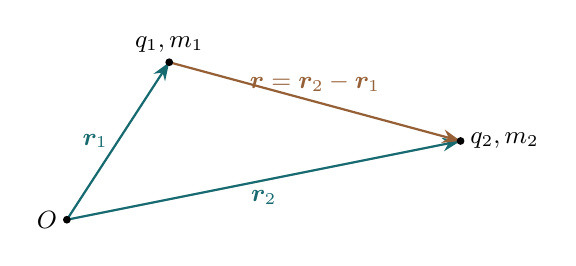
\begin{tikzpicture}[x=1cm,y=1cm]
\coordinate (O) at (0,0);\coordinate (A) at (1.3,2);\coordinate (B) at (5,1);
\draw[motion] (O)--(A) node[midway,left] {$\vect r_1$};\draw[motion] (O)--(B) node[midway,below] {$\vect r_2$};
\draw[force] (A)--(B) node[midway,above] {$\vect r=\vect r_2-\vect r_1$};
\foreach \p in {A,B,O}\fill (\p) circle (1.4pt);
\node[left] at (O) {$O$};\node[above] at (A) {$q_1,m_1$};\node[right] at (B) {$q_2,m_2$};
\end{tikzpicture}\figcaption{图 电1.1　相对位矢从电荷1指向电荷2。}\end{minipage}\end{center}

\workarea

\clearpage

\pdfbookmark[2]{第 2 题 正方形中心电荷的小振动}{q2}

\section*{第 2 题\quad 正方形中心电荷的小振动}\label{q:2}

边长为$a$的正方形四个顶点各固定一个电量为$Q$的点电荷。中心放一个质量为$m$、电量为$q$的自由点电荷，$qQ>0$。将它沿一条对角线移动很小的距离后由静止释放。判断它是否作周期性振动；若是，求小振动周期，并说明稳定性的空间范围。

\begin{center}\begin{minipage}{0.97\linewidth}\centering
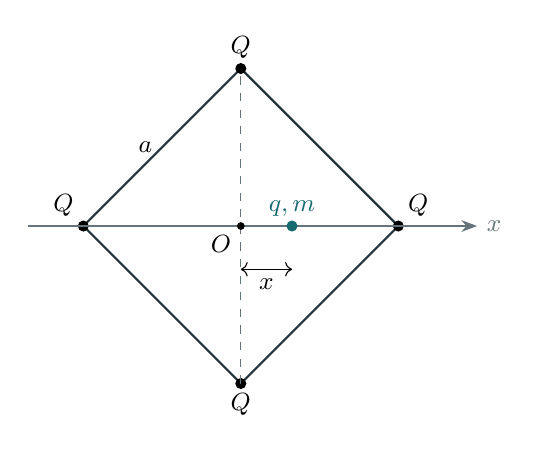
\begin{tikzpicture}[x=1cm,y=1cm]
\draw[object] (-2,0)--(0,2)--(2,0)--(0,-2)--cycle;
\foreach \x/\y in {-2/0,0/2,2/0,0/-2}\fill (\x,\y) circle (2pt);\node[above left] at (-2,0) {$Q$};\node[above] at (0,2) {$Q$};\node[above right] at (2,0) {$Q$};\node[below] at (0,-2) {$Q$};
\draw[axis] (-2.7,0)--(3,0) node[right] {$x$};\draw[guide] (0,-2)--(0,2);
\fill (0,0) circle (1.4pt) node[below left] {$O$};\fill[accent] (.65,0) circle (2pt) node[above] {$q,m$};
\node[left] at (-1,1) {$a$};\draw[<->] (0,-.55)--(.65,-.55) node[midway,below] {$x$};
\end{tikzpicture}\figcaption{图 电1.2　沿水平对角线释放电荷，四个顶点电荷固定。}\end{minipage}\end{center}

\workarea

\clearpage

\pdfbookmark[2]{第 3 题 共线四点电荷作用下的轴向运动}{q3}

\section*{第 3 题\quad 共线四点电荷作用下的轴向运动}\label{q:3}

在$x$轴的$x=\pm a$处各固定一个电量为$Q$的点电荷，在$x=\pm2a$处各固定一个电量为$-8Q$的点电荷，$Q>0$。电量为$q>0$、质量为$m$的质点只能沿$x$轴运动。判断原点$O$是否为稳定平衡位置。若稳定，将质点移至$x=A$处静止释放，$0<A\ll a$，求振动周期的主阶表达式。

\begin{center}\begin{minipage}{0.97\linewidth}\centering
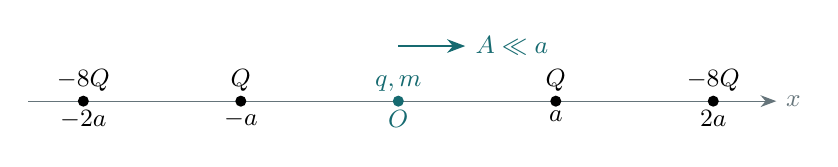
\begin{tikzpicture}[x=1cm,y=1cm]
\draw[axis] (-4.7,0)--(4.8,0) node[right] {$x$};
\foreach \x/\t/\p in {-4/{-8Q}/{-2a},-2/Q/{-a},2/Q/a,4/{-8Q}/{2a}}{\fill (\x,0) circle (2pt);\node[above] at (\x,0) {$\t$};\node[below] at (\x,0) {$\p$};}
\fill[accent] (0,0) circle (2pt) node[above] {$q,m$} node[below] {$O$};
\draw[motion] (0,.7)--(.85,.7) node[right] {$A\ll a$};
\end{tikzpicture}\figcaption{图 电1.3　四个固定电荷共线排列，活动电荷限制在该直线上运动。}\end{minipage}\end{center}

\workarea

\clearpage

\pdfbookmark[2]{第 4 题 反平方律与带电球壳的内场}{q4}

\section*{第 4 题\quad 反平方律与带电球壳的内场}\label{q:4}

证明：若真空中的电力严格服从反平方律，一个孤立带电导体球壳达到静电平衡时，电荷均匀分布在外表面，球壳内部电场处处为零。球形空腔内没有电荷，外部没有其他电荷或外加电场。说明证明中反平方律起什么作用。

\begin{center}\begin{minipage}{0.97\linewidth}\centering
\begin{tikzpicture}[x=1cm,y=1cm]
\fill[accent!10] (0,0) circle (1.9);\fill[white] (0,0) circle (1.45);\draw[object] (0,0) circle (1.9);\draw[object] (0,0) circle (1.45);
\fill (0,0) circle (1pt) node[below] {$O$};\fill (.55,.5) circle (1.5pt) node[above] {$P$};
\foreach \t in {0,45,...,315}\node at (\t:2.08) {$+$};
\node[right,align=left] at (2.8,.35) {球形空腔内无电荷\\外部无其他电荷};
\end{tikzpicture}\figcaption{图 电1.4　孤立导体球壳的静电平衡；图示取总电荷为正。}\end{minipage}\end{center}

\workarea

\clearpage

\pdfbookmark[2]{第 5 题 异号半圆环在轴线上的电场}{q5}

\section*{第 5 题\quad 异号半圆环在轴线上的电场}\label{q:5}

半径为$R$的圆环位于$xy$平面，圆心为原点。电荷线密度在$y<0$的半圆上为$+\lambda_0$，在$y>0$的半圆上为$-\lambda_0$，其中$\lambda_0>0$。求垂直于圆环平面、通过圆心的$z$轴上任意一点的电场。

\begin{center}\begin{minipage}{0.97\linewidth}\centering
\begin{tikzpicture}[x=1cm,y=1cm]
\draw[axis] (-2.4,0)--(2.5,0) node[right] {$x$};\draw[axis] (0,-2.2)--(0,2.3) node[above] {$y$};
\draw[very thick,warm] (-1.7,0) arc (180:360:1.7);\draw[very thick,accent] (1.7,0) arc (0:180:1.7);
\node at (0,-1.1) {$+\lambda_0$};\node at (0,1.1) {$-\lambda_0$};\node[below left] at (0,0) {$O$};
\draw[<->] (0,0)--({1.7/sqrt(2)},{-1.7/sqrt(2)}) node[midway,above] {$R$};\node[right,align=left] at (3,.2) {$z$轴垂直纸面\\观察点$P=(0,0,z)$};
\end{tikzpicture}\figcaption{图 电1.5　俯视圆环：下半环带正电，上半环带负电。}\end{minipage}\end{center}

\workarea

\clearpage

\pdfbookmark[2]{第 6 题 半圆弧与两条半无限直线的电场}{q6}

\section*{第 6 题\quad 半圆弧与两条半无限直线的电场}\label{q:6}

一条均匀带电细线弯成图示形状：左侧$AB$为半圆弧；$AA'$和$BB'$为分别与圆弧相切、向右无限延伸的两条平行直线。求半圆圆心$O$处的电场。可自设圆弧半径$R$和电荷线密度$\lambda$。

\begin{center}\begin{minipage}{0.97\linewidth}\centering
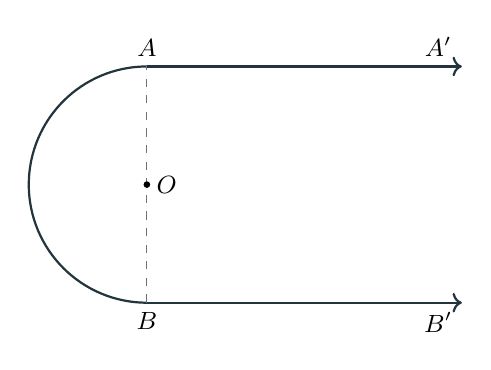
\begin{tikzpicture}[x=1cm,y=1cm]\draw[object] (0,1.5) arc (90:270:1.5);\draw[object,->] (0,1.5)--(4,1.5);\draw[object,->] (0,-1.5)--(4,-1.5);\draw[guide] (0,-1.5)--(0,1.5);\fill (0,0) circle (1.2pt) node[right] {$O$};\node[above] at (0,1.5) {$A$};\node[below] at (0,-1.5) {$B$};\node[above] at (3.7,1.5) {$A'$};\node[below] at (3.7,-1.5) {$B'$};\end{tikzpicture}\figcaption{图 电1.6　两条直线从圆弧端点向右无限延伸，线密度处处相同。}\end{minipage}\end{center}

\workarea

\clearpage

\pdfbookmark[2]{第 7 题 均匀带电半圆环的圆心电场}{q7}

\section*{第 7 题\quad 均匀带电半圆环的圆心电场}\label{q:7}

半径为$R$的半圆环均匀带电，电荷线密度为$\lambda$。半圆环位于$xy$平面内的$x\le0$一侧，圆心为原点$O$。求圆心处的电场，并给出方向。

\begin{center}\begin{minipage}{0.97\linewidth}\centering
\begin{tikzpicture}[x=1cm,y=1cm]
\draw[axis] (-2.2,0)--(2.3,0) node[right] {$x$};\draw[axis] (0,-2)--(0,2) node[above] {$y$};
\draw[very thick,accent] (0,1.6) arc (90:270:1.6);\draw[guide] (0,0)--(135:1.6) node[midway,below] {$R$};
\node[below right] at (0,0) {$O$};\node[left] at (-1.6,0) {$\lambda$};
\end{tikzpicture}\figcaption{图 电1.7　半圆环位于左半平面；电荷符号由线密度给出。}\end{minipage}\end{center}

\workarea

\clearpage

\pdfbookmark[2]{第 8 题 球形区域内电场的体积平均}{q8}

\section*{第 8 题\quad 球形区域内电场的体积平均}\label{q:8}

固定点电荷$5Q$和$12Q$分别位于$A,B$，$AB=13a$。另一点$C$满足$CA=5a$、$CB=12a$。对以$C$为球心的球形区域，定义电场的体积平均
\[\overline{\vect E}=\frac1V\int_V\vect E\,\dd V.\]
分别求球半径为$a$、$10a$时$|\overline{\vect E}|$。注意所求是电场矢量的平均值的大小。

\begin{center}\begin{minipage}{0.97\linewidth}\centering
\begin{tikzpicture}[x=1cm,y=1cm]
\coordinate (C) at (0,0);\coordinate (A) at (-1.5,0);\coordinate (B) at (0,-3.6);
\draw[object] (A)--(C)--(B)--cycle;\draw (0,-.2)--(-.2,-.2)--(-.2,0);
\node[above left=3pt] at (A) {$A,5Q$};\node[right] at (B) {$B,12Q$};\node[above right] at (C) {$C$};
\node[below=3pt] at (-.75,0) {$5a$};\node[right] at (0,-1.8) {$12a$};\node[left] at (-.8,-1.8) {$13a$};
\draw[guide] (C) circle (.3);\draw[guide] (C) circle (3);\node[right] at (2.6,1.65) {$s=10a$};\node at (.7,-.55) {$s=a$};
\end{tikzpicture}\figcaption{图 电1.8　截面中的直角三角形；大球包含A，小球不含任何电荷。}\end{minipage}\end{center}

\workarea

\clearpage

\pdfbookmark[2]{第 9 题 均匀带电球中的偏心球形空腔}{q9}

\section*{第 9 题\quad 均匀带电球中的偏心球形空腔}\label{q:9}

半径为$R$、体电荷密度为$\rho$的均匀带电球体内，挖去一个半径为$R'$的球形区域。大球中心为$O$，空腔中心为$O'$，$\vect a=\overrightarrow{OO'}$，$a+R'<R$。求$O'$处电场，并证明整个空腔内的电场均匀。电荷视为固定分布的给定电荷，按真空库仑定律计算。

\begin{center}\begin{minipage}{0.97\linewidth}\centering
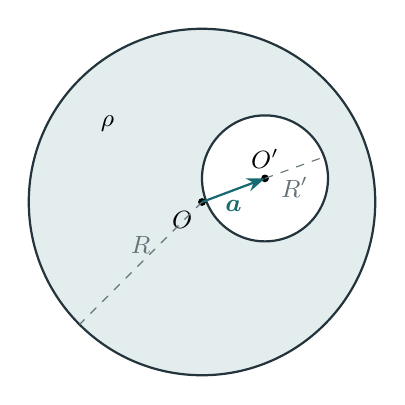
\begin{tikzpicture}[x=1cm,y=1cm]
\fill[accent!12] (0,0) circle (2.2);\fill[white] (.8,.3) circle (.8);\draw[object] (0,0) circle (2.2);\draw[object] (.8,.3) circle (.8);
\fill (0,0) circle (1.4pt) node[below left] {$O$};\fill (.8,.3) circle (1.4pt) node[above] {$O'$};
\draw[motion] (0,0)--(.8,.3) node[midway,below] {$\vect a$};\draw[guide] (0,0)--(225:2.2) node[midway,above] {$R$};
\draw[guide] (.8,.3)--({.8+.8*cos(20)},{.3+.8*sin(20)}) node[midway,below] {$R'$};\node at (-1.2,1) {$\rho$};
\end{tikzpicture}\figcaption{图 电1.9　空腔完全位于大球内部，剩余电荷固定不动。}\end{minipage}\end{center}

\workarea

\clearpage

\pdfbookmark[2]{第 10 题 八分之一带电球体的球心电场}{q10}

\section*{第 10 题\quad 八分之一带电球体的球心电场}\label{q:10}

用三个两两垂直且通过球心的平面，将半径为$R$的球体分成八等份。取第一卦限$x,y,z\ge0$的一份，使其均匀带电，体电荷密度为$\rho$。求球心$O$处电场的大小和方向。

\begin{center}\begin{minipage}{0.97\linewidth}\centering
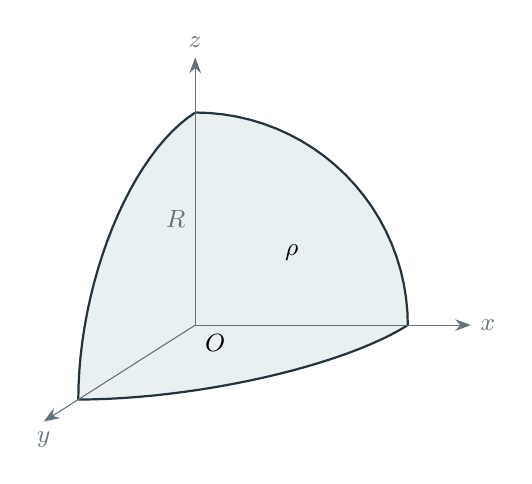
\begin{tikzpicture}[x={(1cm,0cm)},y={(-.55cm,-.35cm)},z={(0cm,1cm)},font=\small]
\fill[accent!10]
plot[domain=0:90,variable=\t] ({2.7*cos(\t)},0,{2.7*sin(\t)})
--plot[domain=90:0,variable=\t] (0,{2.7*cos(\t)},{2.7*sin(\t)})
--plot[domain=90:0,variable=\t] ({2.7*cos(\t)},{2.7*sin(\t)},0)--cycle;
\draw[object,domain=0:90,variable=\t] plot({2.7*cos(\t)},0,{2.7*sin(\t)});
\draw[object,domain=0:90,variable=\t] plot(0,{2.7*cos(\t)},{2.7*sin(\t)});
\draw[object,domain=0:90,variable=\t] plot({2.7*cos(\t)},{2.7*sin(\t)},0);
\draw[axis] (0,0,0)--(3.5,0,0) node[right] {$x$};
\draw[axis] (0,0,0)--(0,3.5,0) node[below] {$y$};
\draw[axis] (0,0,0)--(0,0,3.4) node[above] {$z$};
\draw[guide] (0,0,0)--(0,0,2.7) node[midway,left] {$R$};
\node[below right] at (0,0,0) {$O$};\node at (1.5,.5,1.1) {$\rho$};
\end{tikzpicture}\figcaption{图 电1.10　第一卦限的八分之一球体；三条直边互相垂直。}\end{minipage}\end{center}

\workarea

\clearpage

\pdfbookmark[2]{第 11 题 匀强电场中的连续弹性碰撞}{q11}

\section*{第 11 题\quad 匀强电场中的连续弹性碰撞}\label{q:11}

质量均为$m$的两个小球$A,B$静止在同一直线上，初始间距为$l$。$A$带正电$Q$，$B$不带电；沿$A$指向$B$的方向存在匀强电场$E$。两球发生完全弹性正碰，碰撞时不交换电荷，忽略重力及其他相互作用。证明相邻两次碰撞的时间间隔相同，并求此间隔。

\begin{center}\begin{minipage}{0.97\linewidth}\centering
\begin{tikzpicture}[x=1cm,y=1cm]
\draw[guide] (-.5,0)--(6,0);\fill[accent] (0,0) circle (3pt) node[above] {$A:m,Q$};\fill (4.5,0) circle (3pt) node[above] {$B:m,0$};
\draw[<->] (0,-.7)--(4.5,-.7) node[midway,below] {$l$};\draw[force] (1.2,1)--(3.5,1) node[midway,above] {$\vect E$};
\end{tikzpicture}\figcaption{图 电1.11　两球初始静止；只有A持续受到向右的电力。}\end{minipage}\end{center}

\workarea

\clearpage

\pdfbookmark[2]{第 12 题 带电厚板两侧的分段运动}{q12}

\section*{第 12 题\quad 带电厚板两侧的分段运动}\label{q:12}

无限大均匀带电厚板占据$-d\le x\le d$，体电荷密度为$\rho>0$。质量$m$、电荷$q<0$的质点从$x=2d$处静止释放，仅受厚板的电场力。求它第一次到达厚板中面$x=0$的时间。电荷分布固定，按真空静电定律计算。

\begin{center}\begin{minipage}{0.97\linewidth}\centering
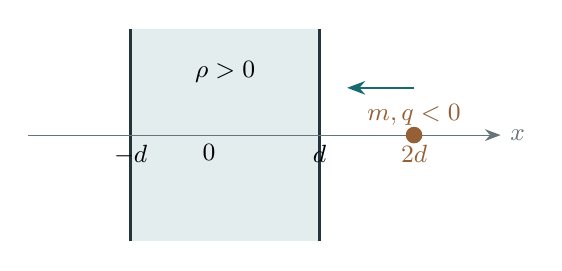
\begin{tikzpicture}[x=1cm,y=1cm]
\fill[accent!12] (-1.2,-1.35) rectangle (1.2,1.35);\draw[object] (-1.2,-1.35)--(-1.2,1.35) (1.2,-1.35)--(1.2,1.35);
\draw[axis] (-2.5,0)--(3.5,0) node[right] {$x$};\node[below] at (-1.2,0) {$-d$};\node[below] at (1.2,0) {$d$};\node[below left] at (0,0) {$0$};\node at (0,.8) {$\rho>0$};
\fill[warm] (2.4,0) circle (3pt) node[above] {$m,q<0$} node[below] {$2d$};\draw[motion] (2.4,.6)--(1.55,.6);
\end{tikzpicture}\figcaption{图 电1.12　粒子先经过板外匀强场，再进入板内线性场。}\end{minipage}\end{center}

\workarea

\clearpage

\pdfbookmark[2]{第 13 题 非均匀带电圆环的平衡与振动}{q13}

\section*{第 13 题\quad 非均匀带电圆环的平衡与振动}\label{q:13}

半径$R$的刚性绝缘细圆环带正电$Q$，电荷可非均匀地固定分布。圆环在$xy$平面内，圆心为$O$。
\begin{enumerate}\item 怎样选择沿圆周的线电荷密度，使一个非零点电荷能沿直径$AOB$的内部作匀速直线运动？以从$+x$轴量起的极角$\phi$表示结果。
\item 将点电荷$Q_1$放在$x=-r_1$，$r_1>R$，已知$|Q_1|=\nu Q$。能否在$x=r_2>R$再放一个点电荷$Q_2$，使两个点电荷与圆环在均无支撑力的情况下同时平衡？求电荷符号、$Q_2,r_2$及参数条件。
\item 固定上述两个点电荷的位置，再把它们同时变号，圆环的电荷不变。圆环质量为$m$，质量分布均匀。将圆环沿$x$轴移动很小的距离$\delta$后静止释放，求其轴向小振动。\end{enumerate}

\begin{center}\begin{minipage}{0.97\linewidth}\centering
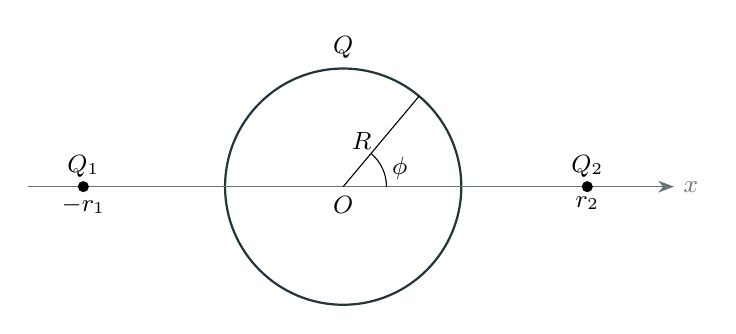
\begin{tikzpicture}[x=1cm,y=1cm]
\draw[object] (0,0) circle (1.5);\draw[axis] (-4,0)--(4.2,0) node[right] {$x$};\node[below] at (0,0) {$O$};
\fill (-3.3,0) circle (2pt) node[above] {$Q_1$} node[below] {$-r_1$};\fill (3.1,0) circle (2pt) node[above] {$Q_2$} node[below] {$r_2$};
\draw (0,0)--(50:1.5) node[midway,left] {$R$};\draw (.55,0) arc (0:50:.55) node[midway,right] {$\phi$};\node[above] at (0,1.5) {$Q$};
\end{tikzpicture}\figcaption{图 电1.13　点电荷位于环面内的一条直径延长线上。}\end{minipage}\end{center}

\workarea

\clearpage

\pdfbookmark[2]{第 14 题 两固定电荷间带电圆环的稳定性}{q14}

\section*{第 14 题\quad 两固定电荷间带电圆环的稳定性}\label{q:14}

半径$R$、质量$m$的均匀带电圆环带正电$q$，环面垂直于$x$轴，圆心可沿$x$轴移动。两个正点电荷$Q$固定在$x=\pm L$。判断圆心位于原点的平衡是否稳定，并在稳定时求轴向小振动周期。临界情形也须讨论。

\begin{center}\begin{minipage}{0.97\linewidth}\centering
\begin{tikzpicture}[x=1cm,y=1cm]
\draw[axis] (-3.7,0)--(4,0) node[right] {$x$};\draw[object] (.3,0) ellipse (.3 and 1.3);\node[above] at (.3,1.3) {$q,m,R$};
\fill (-2.8,0) circle (2pt) node[above] {$Q$} node[below] {$-L$};\fill (2.8,0) circle (2pt) node[above] {$Q$} node[below] {$L$};\node[below left] at (0,0) {$O$};\draw[<->] (0,-.65)--(.3,-.65) node[right] {$x$};
\end{tikzpicture}\figcaption{图 电1.14　环面垂直于两固定点电荷的连线；圆心仅沿轴线运动。}\end{minipage}\end{center}

\workarea

\clearpage

\pdfbookmark[2]{第 15 题 带电粒子束的电场聚焦}{q15}

\section*{第 15 题\quad 带电粒子束的电场聚焦}\label{q:15}

质量为$m$、电荷为$q>0$的粒子，从$P_1=(-R,0)$以同一速率$v_0$沿与$+x$轴成$0<\phi<\pi/2$的各方向射出。设计一个电场，使这些粒子都经过$P_2=(R,0)$。忽略重力和粒子间作用。给出场的形式、轨迹与会聚条件；若采用分区匀强场模型，须说明边界及其物理含义。

\begin{center}\begin{minipage}{0.97\linewidth}\centering
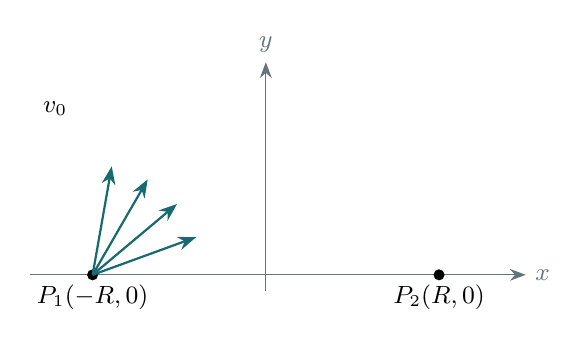
\begin{tikzpicture}[x=1cm,y=1cm]
\draw[axis] (-3,0)--(3.3,0) node[right] {$x$};\draw[axis] (0,-.2)--(0,2.7) node[above] {$y$};
\fill (-2.2,0) circle (2pt) node[below] {$P_1(-R,0)$};\fill (2.2,0) circle (2pt) node[below] {$P_2(R,0)$};
\foreach \a in {20,40,60,80}\draw[motion] (-2.2,0)--++(\a:1.4);\node[above left] at (-2.4,1.9) {$v_0$};
\end{tikzpicture}\figcaption{图 电1.15　同一点以不同仰角射出的等速粒子，要求经过右侧目标点。}\end{minipage}\end{center}

\workarea

\clearpage

\pdfbookmark[2]{第 16 题 两个半球面的底面电势}{q16}

\section*{第 16 题\quad 两个半球面的底面电势}\label{q:16}

两个均匀带电的薄半球面具有同一球心和同一底面平面，分处该平面的两侧，半径为$R_1>R_2$，面电荷密度分别为$\sigma_1,\sigma_2$。求较大半球底面的一条直径$AOB$上各点的电势，取无穷远电势为零。

\begin{center}\begin{minipage}{0.97\linewidth}\centering
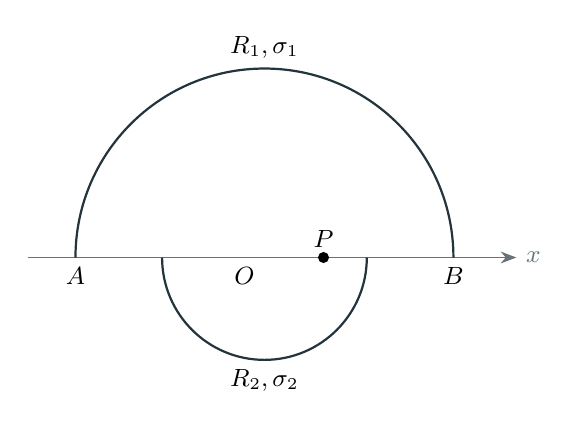
\begin{tikzpicture}[x=1cm,y=1cm]
\draw[axis] (-3,0)--(3.2,0) node[right] {$x$};\draw[object] (2.4,0) arc (0:180:2.4);\draw[object] (-1.3,0) arc (180:360:1.3);
\node[above] at (0,2.4) {$R_1,\sigma_1$};\node[below] at (0,-1.3) {$R_2,\sigma_2$};\node[below] at (-2.4,0) {$A$};\node[below] at (2.4,0) {$B$};\node[below left] at (0,0) {$O$};\fill (.75,0) circle (2pt) node[above] {$P$};
\end{tikzpicture}\figcaption{图 电1.16　沿共同底面的直径观察，两个半球分居底面的两侧。}\end{minipage}\end{center}

\workarea

\clearpage

\pdfbookmark[2]{第 17 题 带电圆环电势的球面平均}{q17}

\section*{第 17 题\quad 带电圆环电势的球面平均}\label{q:17}

半径$R_1$、总电荷$Q$的细圆环，其轴线上有一半径$R_2$的球面，球心到环心距离为$L$。求圆环电荷在该球面上产生的电势的面积平均值。球面只是取平均的几何曲面，不是导体；取无穷远电势为零，并讨论球面包围圆环与不包围圆环的情形。

\begin{center}\begin{minipage}{0.97\linewidth}\centering
\begin{tikzpicture}[x=1cm,y=1cm]
\draw[object] (-2,0) ellipse (.35 and 1.2);\draw[object] (1.5,0) circle (1.5);\draw[guide] (-2.6,0)--(3.5,0);\fill (-2,0) circle (1pt) node[below] {$O$};\fill (1.5,0) circle (1pt) node[below] {$C$};\draw[<->] (-2,-1.8)--(1.5,-1.8) node[midway,below] {$L$};\node[above] at (-2,1.2) {圆环$Q,R_1$};\draw (1.5,0)--++(45:1.5) node[midway,left] {$R_2$};
\end{tikzpicture}\figcaption{图 电1.17　球面用于取面积平均；图示为圆环位于球面外的一种位置。}\end{minipage}\end{center}

\workarea

\clearpage

\pdfbookmark[2]{第 18 题 重力与电力共同作用下的最大速度}{q18}

\section*{第 18 题\quad 重力与电力共同作用下的最大速度}\label{q:18}

地面上固定点电荷$Q$。一个质量为$m$的小带电质点沿经过$Q$的竖直线运动，在距地面$H/2$和$H$的两位置之间往复运动。只计重力与库仑力。求质点运动中的最大速度及达到最大速度的位置。

\begin{center}\begin{minipage}{0.97\linewidth}\centering
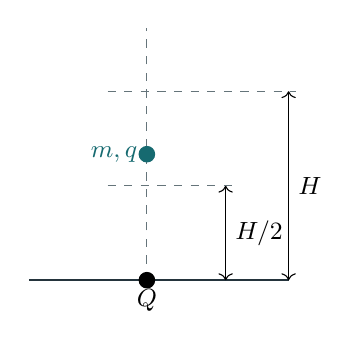
\begin{tikzpicture}[x=1cm,y=1cm]
\draw[object] (-1.5,0)--(1.8,0);\draw[guide] (0,0)--(0,3.2);\fill (0,0) circle (3pt) node[below] {$Q$};\fill[accent] (0,1.6) circle (3pt) node[left] {$m,q$};\draw[<->] (1,0)--(1,1.2) node[midway,right] {$H/2$};\draw[<->] (1.8,0)--(1.8,2.4) node[midway,right] {$H$};\draw[guide] (-.5,1.2)--(1.1,1.2) (-.5,2.4)--(1.9,2.4);
\end{tikzpicture}\figcaption{图 电1.18　两个转向高度分别为H/2和H；小球只作竖直运动。}\end{minipage}\end{center}

\workarea

\clearpage

\pdfbookmark[2]{第 19 题 穿越两个带电球壳的能量门槛}{q19}

\section*{第 19 题\quad 穿越两个带电球壳的能量门槛}\label{q:19}

两个固定的均匀带电球壳，球心为$A,B$，电荷分别为$4Q,Q$，$Q>0$，两球心距离$d$远大于各球壳半径。沿$AB$连线在两球壳上开三个小孔，如图。质量$m$、电荷$-q$（$q>0$）的质点在$A$左侧距$A$为$x$处静止释放。求它穿过三孔并到达$B$球心所需的临界起始距离，说明等于临界值时的运动。忽略小孔对给定均匀电荷分布的影响。

\begin{center}\begin{minipage}{0.97\linewidth}\centering
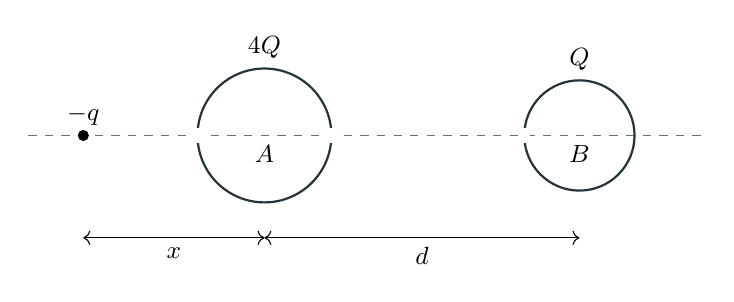
\begin{tikzpicture}[x=1cm,y=1cm]
\draw[guide] (-3,0)--(5.6,0);\draw[object] (0,0) circle (.85);\draw[object] (4,0) circle (.7);\foreach \x in {-.85,.85,3.3}\draw[white,line width=4pt] (\x,-.10)--(\x,.10);\fill (-2.3,0) circle (2pt) node[above] {$-q$};\node[below] at (0,0) {$A$};\node[below] at (4,0) {$B$};\node[above] at (0,.85) {$4Q$};\node[above] at (4,.7) {$Q$};\draw[<->] (-2.3,-1.3)--(0,-1.3) node[midway,below] {$x$};\draw[<->] (0,-1.3)--(4,-1.3) node[midway,below] {$d$};
\end{tikzpicture}\figcaption{图 电1.19　沿轴线穿过A壳两孔和B壳左孔；球壳半径在图中有所放大。}\end{minipage}\end{center}

\workarea

\clearpage

\pdfbookmark[2]{第 20 题 半圆柱电场中的速度选择与聚焦}{q20}

\section*{第 20 题\quad 半圆柱电场中的速度选择与聚焦}\label{q:20}

两个同轴半圆柱电极之间，内、外半径分别为$a,b$，电势为$\varphi(r)=\kappa\ln(b/r)$，$\kappa>0$。质量$m$、电荷$-q$（$q>0$）的粒子垂直轴线射入。
\begin{enumerate}\item 粒子在任意入射半径$\rho$（$a<\rho<b$）沿圆周运动时，其速率应是多少？
\item 若入射方向与该圆周切线偏离很小的角$\beta$，证明在近轴一阶近似下，轨迹第一次重新经过$r=\rho$时对应的方位角与$\rho$及$\beta$无关，并求此角。\end{enumerate}

\begin{center}\begin{minipage}{0.97\linewidth}\centering
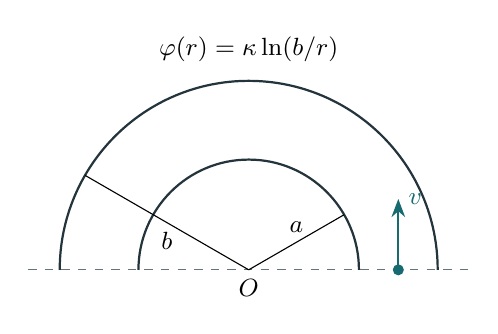
\begin{tikzpicture}[x=1cm,y=1cm]
\draw[object] (2.4,0) arc (0:180:2.4);\draw[object] (1.4,0) arc (0:180:1.4);\draw[guide] (-2.8,0)--(2.8,0);\node[below] at (0,0) {$O$};\draw (0,0)--(30:1.4) node[midway,above] {$a$};\draw (0,0)--(150:2.4) node[midway,below] {$b$};\fill[accent] (1.9,0) circle (2pt);\draw[motion] (1.9,0)--(1.9,.9) node[right] {$v$};\node at (0,2.8) {$\varphi(r)=\kappa\ln(b/r)$};
\end{tikzpicture}\figcaption{图 电1.20　粒子沿圆周切向进入半圆柱电场，径向电力朝向O。}\end{minipage}\end{center}

\workarea

\clearpage

\pdfbookmark[2]{第 21 题 有限线电荷的场线与等势线}{q21}

\section*{第 21 题\quad 有限线电荷的场线与等势线}\label{q:21}

长度$l$的细直线段$AB$均匀带电，线密度$\lambda>0$。取其中点为原点，$AB$为$x$轴。
\begin{enumerate}\item 证明任一轴外点$P$的电场方向沿$\angle APB$的角平分线所在直线，并确定指向。
\item 求包含$AB$的平面内的电场线方程。
\item 求同一平面内的等势线方程。\end{enumerate}

\begin{center}\begin{minipage}{0.97\linewidth}\centering
\begin{tikzpicture}[x=1cm,y=1cm]
\draw[axis] (-3,0)--(3.2,0) node[right] {$x$};\draw[axis] (0,-.3)--(0,2.6) node[above] {$y$};\draw[very thick,accent] (-1.7,0)--(1.7,0);\node[below] at (-1.7,0) {$A$};\node[below] at (1.7,0) {$B$};\node[below left] at (0,0) {$O$};\fill (.8,1.9) circle (2pt) node[above] {$P$};\draw[guide] (-1.7,0)--(.8,1.9)--(1.7,0);\draw[<->] (-1.7,-.8)--(1.7,-.8) node[midway,below] {$l$};
\end{tikzpicture}\figcaption{图 电1.21　以有限线段的两个端点为几何焦点。}\end{minipage}\end{center}

\workarea

\clearpage

\pdfbookmark[2]{第 22 题 两等量点电荷的径向场与切向场}{q22}

\section*{第 22 题\quad 两等量点电荷的径向场与切向场}\label{q:22}

在$x$轴的$x=\pm a$处分别固定电量为$Q\ne0$的点电荷。求$xy$平面内电场相对于原点$O$恰沿径向的点的轨迹，以及恰沿切向的点的轨迹。在场强非零的位置，以整个场强矢量定义方向。轨迹取原点和两处点电荷之外的点。

\begin{center}\begin{minipage}{0.97\linewidth}\centering
\begin{tikzpicture}[x=1cm,y=1cm]
\draw[axis] (-3,0)--(3.3,0) node[right] {$x$};\draw[axis] (0,-1)--(0,2.3) node[above] {$y$};\foreach \x/\t in {-1.8/{-a},1.8/a}{\fill (\x,0) circle (2pt) node[above] {$Q$} node[below] {$\t$};}\fill (1,1.4) circle (2pt) node[right] {$P$};\draw[motion] (0,0)--(1,1.4) node[midway,left] {$\vect r$};
\end{tikzpicture}\figcaption{图 电1.22　径向和切向均相对于原点O定义。}\end{minipage}\end{center}

\workarea

\clearpage

\pdfbookmark[2]{第 23 题 异号平行线电荷的等势面与场线}{q23}

\section*{第 23 题\quad 异号平行线电荷的等势面与场线}\label{q:23}

两条平行无限长直线分别带均匀线电荷密度$+\lambda,-\lambda$（$\lambda>0$），间距$2a$。取它们垂直$xy$平面，在该平面内分别穿过$(a,0)$与$(-a,0)$。求等势面及电场线的空间分布，取原点电势为零。

\begin{center}\begin{minipage}{0.97\linewidth}\centering
\begin{tikzpicture}[x=1cm,y=1cm]
\draw[axis] (-3,0)--(3.2,0) node[right] {$x$};\draw[axis] (0,-1.3)--(0,1.9) node[above] {$y$};\foreach \x/\lab/\p in {-1.5/{-\lambda}/{-a},1.5/{+\lambda}/a}{\draw[object] (\x,0) circle (.12);\fill (\x,0) circle (1pt);\node[above] at (\x,.2) {$\lab$};\node[below] at (\x,-.1) {$\p$};}\node at (0,-1.8) {两带电直线均沿$z$方向垂直纸面};
\end{tikzpicture}\figcaption{图 电1.23　横截面中正线在右、负线在左，间距为2a。}\end{minipage}\end{center}

\workarea

\clearpage

\pdfbookmark[2]{第 24 题 带电球面的有效场与表面张力}{q24}

\section*{第 24 题\quad 带电球面的有效场与表面张力}\label{q:24}

均匀带电薄球面半径为$R$、总电量为$Q$，真空场能密度为$u=\varepsilon_0E^2/2$。求：\begin{enumerate}\item 作用于球面电荷元的有效电场；\item 若靠球面内的各向同性张力维持平衡，所需表面张力系数。\end{enumerate}区分球面内外的场极限与电荷元所受的场。

\begin{center}\begin{minipage}{0.97\linewidth}\centering
\begin{tikzpicture}[x=1cm,y=1cm]
\draw[object] (0,0) circle (1.65);\foreach \a in {0,40,...,320}\node at (\a:1.88) {$+$};\fill (0,0) circle (1pt) node[below] {$O$};\draw (0,0)--(30:1.65) node[midway,above] {$R$};\node[right,align=left] at (2.6,.4) {$Q$固定\\$u=\varepsilon_0E^2/2$};
\end{tikzpicture}\figcaption{图 电1.24　球面电荷产生向外的电压力，膜张力负责平衡。}\end{minipage}\end{center}

\workarea

\clearpage

\pdfbookmark[2]{第 25 题 多个带正电导体的表面电荷}{q25}

\section*{第 25 题\quad 多个带正电导体的表面电荷}\label{q:25}

1998个半径相同、总正电荷相同的导体球彼此不接触，外部没有其他电荷或外加电场。证明达到静电平衡时，至少有一个球的表面处处没有负电荷。

\begin{center}\begin{minipage}{0.97\linewidth}\centering
\begin{tikzpicture}[x=1cm,y=1cm]
\foreach \x/\y/\t in {0/0/1,2/1/2,4/-.1/3,6/1.1/N}{\draw[object] (\x,\y) circle (.55);\node at (\x,\y) {$+Q$};\node[below] at (\x,{\y-.6}) {$\t$};}\node at (3,-1.5) {$N=1998$，各球互不接触};
\end{tikzpicture}\figcaption{图 电1.25　每球净电荷为正，但面密度可能不均匀。}\end{minipage}\end{center}

\workarea

\clearpage

\pdfbookmark[2]{第 26 题 偏心粒子束给金属球充电}{q26}

\section*{第 26 题\quad 偏心粒子束给金属球充电}\label{q:26}

加速器使每个质子获得动能$E$。一束很细、很稀的质子束射向远处半径$r$的孤立金属球并被吸收；入射直线到球心的垂直距离为$d<r$。忽略单个粒子的感应效应，球外场可按球心点电荷处理。求充电停止时的球电势，并计算$E=2\,\mathrm{keV},d=r/2$时的数值。改用同动能电子时如何变化？

\begin{center}\begin{minipage}{0.97\linewidth}\centering
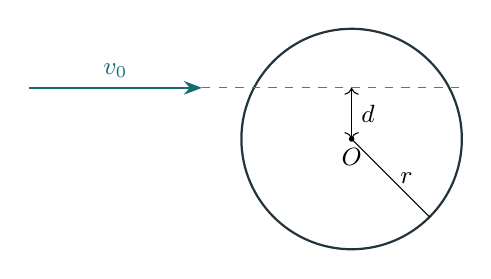
\begin{tikzpicture}[x=1cm,y=1cm]
\draw[object] (2.1,0) circle (1.4);\fill (2.1,0) circle (1pt) node[below] {$O$};\draw[motion] (-2,.65)--(.2,.65) node[midway,above] {$v_0$};\draw[guide] (.2,.65)--(3.5,.65);\draw[<->] (2.1,0)--(2.1,.65) node[midway,right] {$d$};\draw (2.1,0)--++(-45:1.4) node[midway,right] {$r$};
\end{tikzpicture}\figcaption{图 电1.26　入射束流不穿过球心，碰撞参数为d。}\end{minipage}\end{center}

\workarea

\clearpage

\pdfbookmark[2]{第 27 题 三导体球的电势、电荷与空间电场}{q27}

\section*{第 27 题\quad 三导体球的电势、电荷与空间电场}\label{q:27}

导体球$A,B,C$半径分别为$2\,\mathrm{cm},2\,\mathrm{cm},3\,\mathrm{cm}$，球心组成边长$s=50\,\mathrm{cm}$的等边三角形。开始时各球电荷为$12,24,30\,\mathrm{nC}$。
\begin{enumerate}\item 近似求$B$球电势，估计近似的误差。
\item 用细导线连接三球，忽略导线上的电荷，求平衡后的各球电荷。
\item 设三角形中心为$O$，取$+x$轴垂直三角形平面，$+y$轴在该平面内由$C$指向$O$。求连接后$P=(OC,0,0)$处的电场大小和方向。\end{enumerate}

\begin{center}\begin{minipage}{0.97\linewidth}\centering
\begin{tikzpicture}[x=1cm,y=1cm]
\coordinate (A) at (2,0);\coordinate (B) at (-2,0);\coordinate (C) at (0,{2*sqrt(3)});\draw[guide] (A)--(B)--(C)--cycle;\foreach \p in {A,B}\draw[object] (\p) circle (.16);\draw[object] (C) circle (.24);\node[below=8pt] at (A) {$A:2\,\mathrm{cm}$};\node[below=8pt] at (B) {$B:2\,\mathrm{cm}$};\node[above=11pt] at (C) {$C:3\,\mathrm{cm}$};\fill (0,{2*sqrt(3)/3}) circle (1.5pt) node[right] {$O$};\node[below] at (0,0) {$s=50\,\mathrm{cm}$};
\end{tikzpicture}\figcaption{图 电1.27　三球心构成等边三角形，球半径与间距按同一比例表示。}\end{minipage}\end{center}

\workarea

\clearpage

\pdfbookmark[2]{第 28 题 四个导体球依次连接后的电荷}{q28}

\section*{第 28 题\quad 四个导体球依次连接后的电荷}\label{q:28}

四个半径均为$a$的相同导体球，球心位于边长$r$的正方形四个顶点，按图依次编号1、2、3、4，$r\gg a$。起初只有球1带电$Q>0$，其余不带电。用细金属丝把球1依次与球2、3、4连接，每次达到静电平衡后再断开。忽略金属丝带电，求四球最终电荷，保留相互影响的一阶修正。

\begin{center}\begin{minipage}{0.97\linewidth}\centering
\begin{tikzpicture}[x=1cm,y=1cm]
\draw[guide] (0,0)--(3,0)--(3,3)--(0,3)--cycle;\foreach \x/\y/\t in {0/3/1,3/3/2,3/0/3,0/0/4}{\draw[object] (\x,\y) circle (.23);\node[above right=5pt] at (\x,\y) {$\t$};}\node[right] at (3,1.5) {$r$};\node[left] at (0,1.5) {球半径$a\ll r$};
\end{tikzpicture}\figcaption{图 电1.28　球1依次与2、3、4连接，每次稳态后断开。}\end{minipage}\end{center}

\workarea

\clearpage

\pdfbookmark[2]{第 29 题 移去三角形的一根带电细棒}{q29}

\section*{第 29 题\quad 移去三角形的一根带电细棒}\label{q:29}

三根等长绝缘细棒首尾相接构成等边三角形$abc$，棒上固定的电荷分布与同形状孤立导体框静电平衡时的分布相同。$A$为三角形中心，$B$为$A$关于边$bc$的镜像点。已测得电势$U_A,U_B$。所有电势均以无穷远为零。移走棒$ab$，其余两棒电荷分布不变，求此时$A,B$两点的电势。

\begin{center}\begin{minipage}{0.97\linewidth}\centering
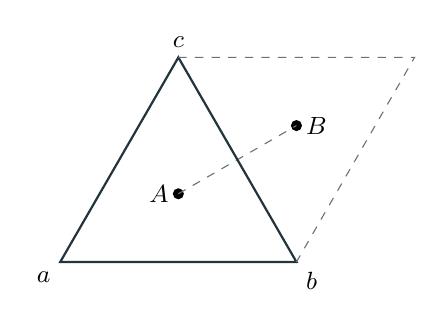
\begin{tikzpicture}[x=1cm,y=1cm]\coordinate (a) at (0,0);\coordinate (b) at (3,0);\coordinate (c) at (1.5,{1.5*sqrt(3)});\coordinate (A) at (1.5,{sqrt(3)/2});\coordinate (B) at (3,{sqrt(3)});\node[below left] at (a) {$a$};\node[below right] at (b) {$b$};\node[above] at (c) {$c$};\fill (A) circle (2pt) node[left] {$A$};\fill (B) circle (2pt) node[right] {$B$};\draw[guide] (A)--(B);\draw[object] (a)--(b)--(c)--cycle;\draw[guide] (c)--(4.5,{1.5*sqrt(3)})--(b);\end{tikzpicture}\figcaption{图 电1.29　B是中心A关于边bc的镜像。}\end{minipage}\end{center}

\workarea

\clearpage

\pdfbookmark[2]{第 30 题 带电隔板与等温气体的平衡}{q30}

\section*{第 30 题\quad 带电隔板与等温气体的平衡}\label{q:30}

恒温矩形容器的两端为面积$A$、相距$2L$的接地金属板，其余壁绝缘。面积也为$A$的可动金属隔板带固定总电荷$Q$，将两侧理想气体隔开；隔板居中时，两侧压强均为$p_0$。隔板无摩擦、不漏气，气体经历准静态等温过程，忽略边缘场及隔板厚度。求全部平衡位置，并讨论稳定性，包括临界参数情形。

\begin{center}\begin{minipage}{0.97\linewidth}\centering
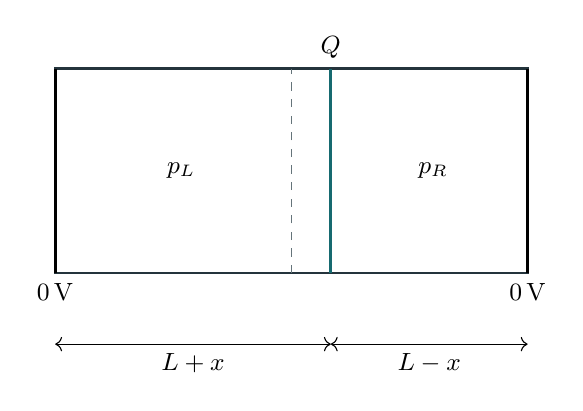
\begin{tikzpicture}[x=1cm,y=1cm]
\draw[object] (0,0) rectangle (6,2.6);\draw[very thick] (0,0)--(0,2.6) (6,0)--(6,2.6);\draw[very thick,accent] (3.5,0)--(3.5,2.6);\node at (1.6,1.3) {$p_L$};\node at (4.8,1.3) {$p_R$};\node[above] at (3.5,2.6) {$Q$};\node[below] at (0,0) {$0\,\mathrm V$};\node[below] at (6,0) {$0\,\mathrm V$};\draw[<->] (0,-.9)--(3.5,-.9) node[midway,below] {$L+x$};\draw[<->] (3.5,-.9)--(6,-.9) node[midway,below] {$L-x$};\draw[guide] (3,0)--(3,2.6);
\end{tikzpicture}\figcaption{图 电1.30　两端固定板接地，移动隔板带固定总电荷Q。}\end{minipage}\end{center}

\workarea

\clearpage

\pdfbookmark[2]{第 31 题 同轴电极间的离子迁移与补充电荷}{q31}

\section*{第 31 题\quad 同轴电极间的离子迁移与补充电荷}\label{q:31}

半径$R$的接地长金属圆筒内，有一根半径$r_0$的同轴细导线，导线电势保持$U_0>0$。导线附近介质电离，电子被导线吸附，正离子形成均匀同轴薄圆柱层向外迁移，迁移率$w=v_r/E$为常量。
\begin{enumerate}\item 忽略电离引起的场变化，证明离子层位置满足$r^2=\kappa(t+t_0)$，求$\kappa,t_0$。
\item 若该离子层总电荷为$Q$，从电离开始计时，求为保持导线电势不变而由电源补充的正电荷$Q^*(t)$，直到离子到达外筒。\end{enumerate}

\begin{center}\begin{minipage}{0.97\linewidth}\centering
\begin{tikzpicture}[x=1cm,y=1cm]
\draw[object] (0,0) circle (1.9);\fill[ink!20] (0,0) circle (.22);\draw[object] (0,0) circle (.22);\draw[accent,thick] (0,0) circle (1);\draw (0,0)--(35:1.9) node[midway,above] {$R$};\draw (0,0)--(145:1) node[midway,above] {$r(t)$};\node[below] at (0,-.3) {$r_0,U_0$};\node[right] at (2.3,0) {外筒接地};
\end{tikzpicture}\figcaption{图 电1.31　正离子薄层沿径向外移，导线保持正电势。}\end{minipage}\end{center}

\workarea

\clearpage

\pdfbookmark[2]{第 32 题 点电荷附近导体薄板的感应电荷}{q32}

\section*{第 32 题\quad 点电荷附近导体薄板的感应电荷}\label{q:32}

半径$R$的圆形导体薄板，其轴线上距板心$a$处固定点电荷$Q$，$a\ll R$。分别讨论薄板接地和薄板孤立且总电荷为$Q_0$时，两面的电荷分布。先在忽略边缘效应的平板近似下求解，并说明这一近似对有限圆盘的适用范围。

\begin{center}\begin{minipage}{0.97\linewidth}\centering
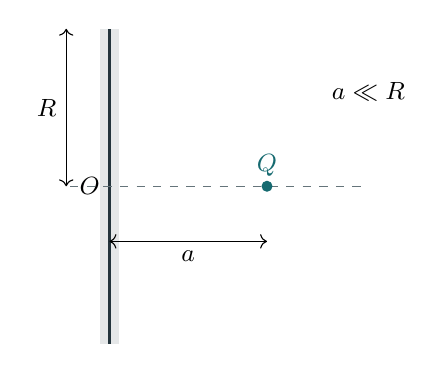
\begin{tikzpicture}[x=1cm,y=1cm]
\fill[ink!12] (-.12,-2) rectangle (.12,2);\draw[object] (0,-2)--(0,2);\draw[guide] (-.5,0)--(3.2,0);\fill[accent] (2,0) circle (2pt) node[above] {$Q$};\node[left] at (0,0) {$O$};\draw[<->] (0,-.7)--(2,-.7) node[midway,below] {$a$};\draw[<->] (-.55,0)--(-.55,2) node[midway,left] {$R$};\node[right] at (2.7,1.2) {$a\ll R$};
\end{tikzpicture}\figcaption{图 电1.32　圆盘侧视图，轴向距离局部放大；中心附近可先按平面近似求感应分布。}\end{minipage}\end{center}

\workarea

\clearpage

\pdfbookmark[2]{第 33 题 两接地平面之间的带电摆球}{q33}

\section*{第 33 题\quad 两接地平面之间的带电摆球}\label{q:33}

两块足够大的接地导体平面竖直平行放置，间距$2d$，$d=10\,\mathrm{cm}$。中央悬挂长$l=1\,\mathrm m$的绝缘细线，下系质量$m=0.1\,\mathrm g$、电量$q=5\times10^{-9}\,\mathrm C$的小球。令小球在垂直两板的竖直平面内作小角度摆动，忽略空气阻尼和电磁阻尼。求周期，并给出中央位置稳定的条件。

\begin{center}\begin{minipage}{0.97\linewidth}\centering
\begin{tikzpicture}[x=1cm,y=1cm]
\draw[very thick] (-1.4,-.2)--(-1.4,3.3) (1.4,-.2)--(1.4,3.3);\draw[object] (-.5,3)--(.5,3);\draw[object] (0,3)--(.3,.7);\fill[accent] (.3,.7) circle (3pt) node[right] {$m,q$};\draw[guide] (0,3)--(0,.5);\node[left] at (.05,1.9) {$l$};\draw[<->] (-1.4,-.7)--(0,-.7) node[midway,below] {$d$};\draw[<->] (0,-.7)--(1.4,-.7) node[midway,below] {$d$};\node at (0,-1.5) {两板均接地};
\end{tikzpicture}\figcaption{图 电1.33　小球在垂直两板的竖直平面内小角度摆动，横向间距放大表示。}\end{minipage}\end{center}

\workarea

\clearpage

\pdfbookmark[2]{第 34 题 同号点电荷与带电导体球的吸引}{q34}

\section*{第 34 题\quad 同号点电荷与带电导体球的吸引}\label{q:34}

半径$R$的孤立导体球带总电荷$Q>0$。在距球心$a>R$处放置同号点电荷$q>0$。求两者相互吸引时$q$的取值范围。

\begin{center}\begin{minipage}{0.97\linewidth}\centering
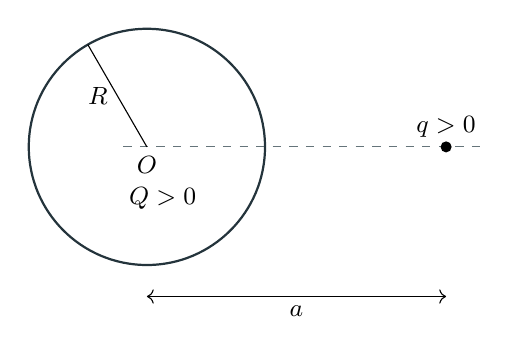
\begin{tikzpicture}[x=1cm,y=1cm]
\draw[object] (0,0) circle (1.5);\node at (.2,-.65) {$Q>0$};\draw[guide] (-.3,0)--(4.3,0);\fill (3.8,0) circle (2pt) node[above] {$q>0$};\node[below] at (0,0) {$O$};\draw (0,0)--(120:1.5) node[midway,left] {$R$};\draw[<->] (0,-1.9)--(3.8,-1.9) node[midway,below] {$a$};
\end{tikzpicture}\figcaption{图 电1.34　孤立导体球与同号点电荷；表面电荷可以重新分布。}\end{minipage}\end{center}

\workarea

\clearpage

\pdfbookmark[2]{第 35 题 两个相切导体球的电容}{q35}

\section*{第 35 题\quad 两个相切导体球的电容}\label{q:35}

两个半径均为$R$的导体球相切，组成一个孤立导体。求它相对于无穷远的电容。忽略连接处的微观结构。

\begin{center}\begin{minipage}{0.97\linewidth}\centering
\begin{tikzpicture}[x=1cm,y=1cm]
\draw[object] (-1.5,0) circle (1.5) (1.5,0) circle (1.5);\fill (-1.5,0) circle (1.5pt) node[below] {$O_1$};\fill (1.5,0) circle (1.5pt) node[below] {$O_2$};\draw (-1.5,0)--(-1.5,1.5) node[midway,left] {$R$};\node[below] at (0,0) {$T$};\node at (0,-2) {两球相切，共同电势为$V$，无穷远电势为零};
\end{tikzpicture}\figcaption{图 电1.35　两等大导体球在T点接触，组成一个孤立导体。}\end{minipage}\end{center}

\workarea

\clearpage

\pdfbookmark[2]{第 36 题 静电互易关系与电容的线性}{q36}

\section*{第 36 题\quad 静电互易关系与电容的线性}\label{q:36}

在$n$个固定且互异的位置分别放置点电荷$q_1,\ldots,q_n$，各点由其他电荷产生的电势为$U_1,\ldots,U_n$；在同样的位置换成$q'_1,\ldots,q'_n$时，相应电势为$U'_1,\ldots,U'_n$。证明
\[\sum_{i=1}^n q_iU'_i=\sum_{i=1}^n q'_iU_i.\]
再据此证明：几何形状和相对位置固定的真空两导体电容器，其电容与带电量无关。两种状态均取无穷远为电势零点。

\begin{center}\begin{minipage}{0.97\linewidth}\centering
\begin{tikzpicture}[x=1cm,y=1cm]
\coordinate (A) at (0,0);\coordinate (B) at (3,0);\coordinate (C) at (1.2,2);\draw[guide] (A)--(B)--(C)--cycle;\foreach \p/\i in {A/1,B/2,C/3}{\fill (\p) circle (2pt);\node[above left] at (\p) {$\i$};}\node at (1.5,-.6) {$q_i\longrightarrow q'_i$};\node[right,align=left] at (4,1) {位置固定\\电荷量改变};
\end{tikzpicture}\figcaption{图 电1.36　互易关系比较同一组固定位置上的两种电荷状态。}\end{minipage}\end{center}

\workarea

\clearpage

\pdfbookmark[2]{第 37 题 带电液珠给电容器逐次充电}{q37}

\section*{第 37 题\quad 带电液珠给电容器逐次充电}\label{q:37}

水平平行金属板$A,B$相距$d$，组成电容为$C$的电容器。上板$B$接地，中间开一小孔；下板$A$孤立。起初两板不带电。在小孔上方$h>0$处，带非零电量$q$、质量$m$的小液珠依次从静止下落，经孔到达$A$即被吸收。前一滴被吸收并达到静电平衡后，下一滴才释放。忽略边缘场、液珠引起的附加感应场和阻力，求能落到$A$的液珠总数。

\begin{center}\begin{minipage}{0.97\linewidth}\centering
\begin{tikzpicture}[x=1cm,y=1cm]
\draw[very thick] (-2,1)--(-.17,1) (.17,1)--(2,1) (-2,-1.2)--(2,-1.2);\node[right] at (2,1) {$B$（接地）};\node[right] at (2,-1.2) {$A$（绝缘）};\fill[accent] (0,2.7) circle (3pt) node[right] {$m,q$};\draw[guide] (0,2.5)--(0,-1);\draw[<->] (-1,1)--(-1,2.7) node[midway,left] {$h$};\draw[<->] (-1,1)--(-1,-1.2) node[midway,left] {$d$};\node at (.8,0) {$C$};
\end{tikzpicture}\figcaption{图 电1.37　同样的带电液珠逐滴下落，上板小孔允许液珠进入板间。}\end{minipage}\end{center}

\workarea

\clearpage

\pdfbookmark[2]{第 38 题 并联电容器错位后的悬浮微粒}{q38}

\section*{第 38 题\quad 并联电容器错位后的悬浮微粒}\label{q:38}

两个相同的水平平行板空气电容器$A,B$并联。充电后，$A$中一带电微粒恰好悬浮。撤去电源，保留两电容器间的连线，把$B$的两极板水平错开，使重叠面积减为原来的一半，板间距不变。忽略边缘效应和微粒对电场的影响，求重新达到电平衡后微粒的加速度。

\begin{center}\begin{minipage}{0.97\linewidth}\centering
\begin{tikzpicture}[x=1cm,y=1cm]
\draw[object] (0,2)--(1.3,2) (1.3,2)--(1.3,1.2) (1.3,.8)--(1.3,0)--(0,0);\draw[object] (.8,1.2)--(1.8,1.2) (.8,.8)--(1.8,.8);\draw[object] (0,2)--(4.3,2)--(4.3,1.2) (0,0)--(4.3,0)--(4.3,.8);\draw[object] (3.8,1.2)--(4.8,1.2) (3.8,.8)--(4.8,.8);\fill[accent] (1.3,1) circle (1.4pt);\node[left] at (.6,1) {$A$};\node[right] at (5,1) {$B$};\node at (2.6,-.6) {电源断开，两电容器仍并联};
\end{tikzpicture}\figcaption{图 电1.38　初态两电容器相同，A中的微粒悬浮。}\end{minipage}\end{center}

\workarea

\clearpage

\pdfbookmark[2]{第 39 题 金属薄板下落产生的电流}{q39}

\section*{第 39 题\quad 金属薄板下落产生的电流}\label{q:39}

边长$L$、板间距$D$的竖直正方形平行板电容器，接在电压恒为$V_0$的电源两端。右板经电流计接地，约定通过电流计向下的电流为正。长为$L$（垂直图面）、高为$L'\ll L$、厚为$D/P$（$P\gg1$）的中性金属板，沿电容器中线从静止下落，起初下端与电容器上沿齐平。忽略边缘效应及电场力对下落的影响。求极板电荷量$Q(t)$并画出$I(t)$。

\begin{center}\begin{minipage}{0.97\linewidth}\centering
\begin{tikzpicture}[x=1cm,y=1cm]
\draw[very thick] (-1.2,-1.7)--(-1.2,1.7) (1.2,-1.7)--(1.2,1.7);\fill[accent!15] (-.28,1.7) rectangle (.28,3);\draw[object] (-.28,1.7) rectangle (.28,3);\draw[motion] (0,3.8)--(0,3.15) node[right] {$g$};\draw[<->] (-1.9,-1.7)--(-1.9,1.7) node[midway,left] {$L$};\draw[<->] (.6,1.7)--(.6,3) node[midway,right] {$L'$};\draw[<->] (-1.2,-2.1)--(1.2,-2.1) node[midway,below] {$D$};\draw[object] (-1.2,0)--(-2.8,0)--(-2.8,-3)--(-.15,-3) (.15,-3)--(2.8,-3)--(2.8,-1.45) (2.8,-.95)--(2.8,0)--(1.2,0);\draw[object] (-.15,-3.3)--(-.15,-2.7) (.15,-3.17)--(.15,-2.83);\node[below] at (0,-3.35) {$V_0$};\draw[object] (1.4,-3)--(1.4,-3.55) (1.15,-3.55)--(1.65,-3.55) (1.22,-3.65)--(1.58,-3.65) (1.29,-3.75)--(1.51,-3.75);\draw[object] (2.8,-1.2) circle (.25);\node at (2.8,-1.2) {G};\draw[motion] (3.5,-.4)--(3.5,-1.3) node[right] {$I>0$};\node[right] at (1.8,2.7) {金属厚度$D/P$};
\end{tikzpicture}\figcaption{图 电1.39　金属板从上方自由下落；电源使两极板电压保持$V_0$。}\end{minipage}\end{center}

\workarea

\clearpage

\pdfbookmark[2]{第 40 题 三个电容器反复换接的电压与热量}{q40}

\section*{第 40 题\quad 三个电容器反复换接的电压与热量}\label{q:40}

电路如图，电源电动势为$\mathcal E$，三个电容器$C_1,C_2,C_3$的电容都为$C$，电阻分别为$R_1,R_2>0$。起初三个电容器都不带电。开关先接$Oa$，再接$Ob$，如此反复；每次均待电路达到稳态后才换接。
\begin{enumerate}\item 第$n$次接$Ob$并达到稳态时，三个电容器的电压各是多少？
\item 无限次换接后，两电阻消耗的总电能是多少？\end{enumerate}

\begin{center}\begin{minipage}{0.97\linewidth}\centering
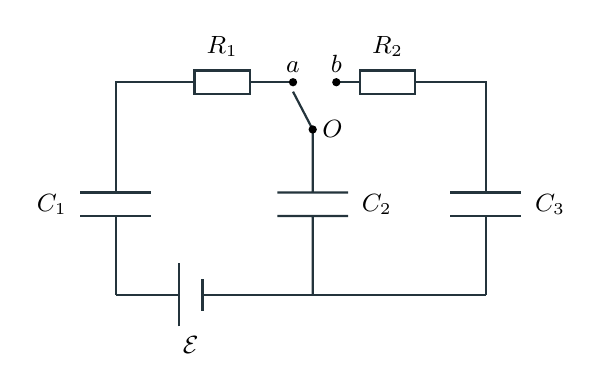
\begin{tikzpicture}[x=1cm,y=1cm]
\draw[object] (0,0)--(0,1) (-.45,1)--(.45,1) (-.45,1.3)--(.45,1.3) (0,1.3)--(0,2.7)--(1,2.7) (1,2.55) rectangle (1.7,2.85);\draw[object] (1.7,2.7)--(2.25,2.7);\fill (2.25,2.7) circle (1.5pt) node[above] {$a$};\draw[object] (4.7,0)--(4.7,1) (4.25,1)--(5.15,1) (4.25,1.3)--(5.15,1.3) (4.7,1.3)--(4.7,2.7)--(3.8,2.7) (3.1,2.55) rectangle (3.8,2.85);\draw[object] (3.1,2.7)--(2.8,2.7);\fill (2.8,2.7) circle (1.5pt) node[above] {$b$};\draw[object] (2.5,0)--(2.5,1) (2.05,1)--(2.95,1) (2.05,1.3)--(2.95,1.3) (2.5,1.3)--(2.5,2.1)--(2.25,2.58);\fill (2.5,2.1) circle (1.5pt) node[right] {$O$};\draw[object] (0,0)--(.8,0) (1.1,0)--(4.7,0);\draw[object] (.8,-.4)--(.8,.4) (1.1,-.2)--(1.1,.2);\node[below] at (.95,-.4) {$\mathcal E$};\node[left] at (-.5,1.15) {$C_1$};\node[right] at (3,1.15) {$C_2$};\node[right] at (5.2,1.15) {$C_3$};\node[above] at (1.35,2.9) {$R_1$};\node[above] at (3.45,2.9) {$R_2$};\end{tikzpicture}\figcaption{图 电1.40　开关每次接到a或b后，都等待电流完全衰减。}\end{minipage}\end{center}

\workarea

\clearpage

\pdfbookmark[2]{第 41 题 略微倾斜的介质电容器}{q41}

\section*{第 41 题\quad 略微倾斜的介质电容器}\label{q:41}

长$a$、宽$b$的两块导体平板略微倾斜，一对宽边间距为$d$，另一对宽边间距为$d+h$，$0<h\ll d$。板间充满相对介电常数$\varepsilon_r$的均匀介质。忽略边缘效应，求电容，保留能体现倾斜影响的近似项。

\begin{center}\begin{minipage}{0.97\linewidth}\centering
\begin{tikzpicture}[x=1cm,y=1cm]
\draw[very thick] (0,0)--(5,0) (0,1.1)--(5,2.2);\draw[<->] (-.5,0)--(-.5,1.1) node[midway,left] {$d$};\draw[<->] (5.5,0)--(5.5,2.2) node[midway,right] {$d+h$};\draw[<->] (0,-.5)--(5,-.5) node[midway,below] {$a$};\node at (2.4,.8) {$\varepsilon_r$};\node at (2.5,2.7) {垂直纸面宽度$b$};
\end{tikzpicture}\figcaption{图 电1.41　一端间距d，另一端间距d＋h，介质充满板间；倾斜放大示意。}\end{minipage}\end{center}

\workarea

\clearpage

\pdfbookmark[2]{第 42 题 同轴圆筒间粒子的绕行与下落}{q42}

\section*{第 42 题\quad 同轴圆筒间粒子的绕行与下落}\label{q:42}

两个同轴竖直导体圆筒，内筒半径$R$，筒间窄缝宽$d$，筒高$L$，$L\gg R\gg d$。内筒经未知电容$C_x$接电压为$V$的电源正极，外筒接负极。窄缝内的$A,B$在同一竖直线上，$B$低于$A$的高度为$h$。质量$m$、电荷$-Q$（$Q>0$）的粒子从$A$水平沿圆周切向射出。求在窄缝圆周运动近似下，使粒子经过$B$的全部$v_0,C_x$组合，并给出允许的整数范围。取两电容间连接节点的初始净电荷为零。忽略端部效应及粒子对电极电荷的影响。

\begin{center}\begin{minipage}{.97\linewidth}\centering
\begin{tikzpicture}[x=1cm,y=1cm,font=\small]
\draw[object] (0,1.8) ellipse (1.6 and .35);
\draw[object] (0,-1.8) ellipse (1.6 and .35);
\draw[object] (-1.6,1.8)--(-1.6,-1.8) (1.6,1.8)--(1.6,-1.8);
\draw[object] (0,1.8) ellipse (1.1 and .25);
\draw[object] (0,-1.8) ellipse (1.1 and .25);
\draw[object] (-1.1,1.8)--(-1.1,-1.8) (1.1,1.8)--(1.1,-1.8);
\draw[guide] (0,2.3)--(0,-2.3);
\fill[accent] (1.35,1.1) circle(2pt) node[right=7pt] {$A$};
\fill[accent] (1.35,-1.1) circle(2pt) node[right=7pt] {$B$};
\draw[<->] (2.3,-1.1)--(2.3,1.1) node[midway,right] {$h$};
\draw[<->] (-2.2,-1.8)--(-2.2,1.8) node[midway,left] {$L$};
\draw[<->] (0,-2.35)--(1.1,-2.35) node[midway,below] {$R$};
\draw[<->] (1.1,-2.35)--(1.6,-2.35) node[midway,below] {$d$};
\node at (0,.6) {内筒$+$};
\node[above] at (0,2.4) {外筒$-$；A、B位于同一缝内母线};
\end{tikzpicture}
\figcaption{图 电1.42　负粒子从A水平切向射出，B在其正下方。窄缝宽度放大示意；内筒经$C_x$接电源正端。}
\end{minipage}\end{center}


\workarea

\clearpage

\pdfbookmark[2]{第 43 题 分批注入带电水银后的球电势}{q43}

\section*{第 43 题\quad 分批注入带电水银后的球电势}\label{q:43}

金属球壳上方连接一根两端各有活栓的细长玻璃管。玻璃管外包金属箔并接地，上方水银槽接电压$V$的电源正极。每次关闭下活栓、打开上活栓使管充满水银，随后关闭上活栓，移去金属箔，再打开下活栓把水银注入球内；恢复装置后重复操作，直至球充满。起初球不带电。玻璃相对介电常数为$\varepsilon_r$，管内半径$r$，管壁厚$d$，球半径$R$，$R\gg r\gg d$。在忽略杂散电容和漏电的理想模型下，估算最终球电势。

\begin{center}\begin{minipage}{0.97\linewidth}\centering
\begin{tikzpicture}[x=1cm,y=1cm]
\draw[object] (-.45,3)--(-.45,.2) (.45,3)--(.45,.2);\draw[very thick,accent] (-.65,2.7)--(-.65,.6) (.65,2.7)--(.65,.6);\draw[object] (-.6,2.85)--(.6,2.85) (-.6,.35)--(.6,.35);\node[right] at (.8,2.85) {上活栓};\node[right] at (.8,.35) {下活栓};\node[left] at (-.8,1.7) {接地箔};\node at (0,1.6) {汞};\draw[motion] (0,.15)--(0,-.3);\draw[object] (0,-1.5) circle (1.15);\node at (0,-1.5) {$R$};\node at (0,-3) {水银经活栓充电、隔离，再注入绝缘支撑的金属球壳};
\end{tikzpicture}\figcaption{图 电1.43　玻璃管内半径r、壁厚d；箔与水银之间构成同轴电容器。}\end{minipage}\end{center}

\workarea

\clearpage

\pdfbookmark[2]{第 44 题 移动介质界面附近点电荷的功}{q44}

\section*{第 44 题\quad 移动介质界面附近点电荷的功}\label{q:44}

半空间$z<0$充满相对介电常数为$\varepsilon_r$的均匀线性各向同性介质，$z>0$为真空，界面没有自由电荷。点电荷$q$在真空内沿法线从$z=h_1>0$缓慢移到$z=h_2>0$。求外力所做的功。

\begin{center}\begin{minipage}{0.97\linewidth}\centering
\begin{tikzpicture}[x=1cm,y=1cm]
\fill[accent!12] (-3,-1.5) rectangle (3,0);\draw[object] (-3,0)--(3,0);\fill (0,1.1) circle (2pt) node[right] {$q,h_1$};\draw[motion] (0,1.3)--(0,2.4);\draw (0,2.6) circle (2pt) node[right] {$q,h_2$};\node at (2,-.7) {$\varepsilon_r$};\node at (2,.5) {真空};\draw[guide] (0,0)--(0,1.1);
\end{tikzpicture}\figcaption{图 电1.44　点电荷沿界面法线缓慢移动，图示$h_2>h_1$；公式也适用于反向移动。}\end{minipage}\end{center}

\workarea

\clearpage

\pdfbookmark[2]{第 45 题 非均匀介质中的极化电荷}{q45}

\section*{第 45 题\quad 非均匀介质中的极化电荷}\label{q:45}

平板电容器的两极板分别带固定自由面电荷密度$+\sigma_0,-\sigma_0$，板间距$d$。其中充满线性各向同性非均匀介质，沿正极板指向负极板取$x$轴，极化率$\chi_e(x)=\chi_0(1+ax)$。求极化体电荷密度$\rho_b(x)$及介质在$x=0,d$两表面的极化面电荷密度。忽略边缘效应，参数满足整个介质内$1+\chi_e(x)>0$。

\begin{center}\begin{minipage}{0.97\linewidth}\centering
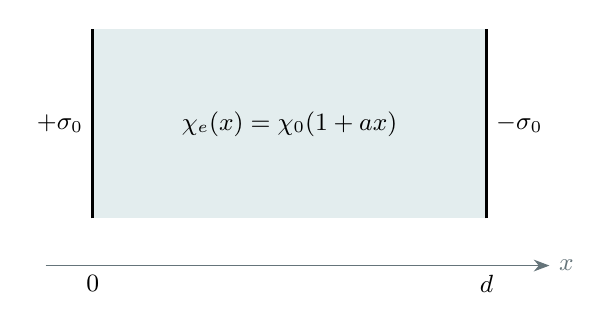
\begin{tikzpicture}[x=1cm,y=1cm]
\fill[accent!12] (0,0) rectangle (5,2.4);\draw[very thick] (0,0)--(0,2.4) (5,0)--(5,2.4);\draw[axis] (-.6,-.6)--(5.8,-.6) node[right] {$x$};\node[below] at (0,-.6) {$0$};\node[below] at (5,-.6) {$d$};\node[left] at (0,1.2) {$+\sigma_0$};\node[right] at (5,1.2) {$-\sigma_0$};\node at (2.5,1.2) {$\chi_e(x)=\chi_0(1+ax)$};
\end{tikzpicture}\figcaption{图 电1.45　自由面电荷固定，介质的极化率随位置变化。}\end{minipage}\end{center}

\workarea

\clearpage

\pdfbookmark[2]{第 46 题 球形电容器的最大耐压}{q46}

\section*{第 46 题\quad 球形电容器的最大耐压}\label{q:46}

同心导体球壳构成球形电容器。外球壳内半径固定为$b=5\,\mathrm{cm}$，内球壳外半径$a$可在$0<a<b$内选择；中间充满均匀各向同性介质，击穿场强$E_b=2.0\times10^7\,\mathrm{V/m}$。求最大可承受电压及对应的内球半径。

\begin{center}\begin{minipage}{0.97\linewidth}\centering
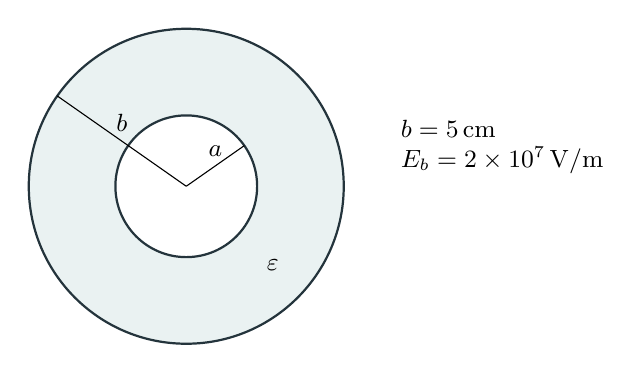
\begin{tikzpicture}[x=1cm,y=1cm]
\fill[accent!9] (0,0) circle (2);\fill[white] (0,0) circle (.9);\draw[object] (0,0) circle (2) (0,0) circle (.9);\draw (0,0)--(35:.9) node[midway,above] {$a$};\draw (0,0)--(145:2) node[midway,above] {$b$};\node at (1.1,-1) {$\varepsilon$};\node[right,align=left] at (2.6,.5) {$b=5\,\mathrm{cm}$\\$E_b=2\times10^7\,\mathrm{V/m}$};
\end{tikzpicture}\figcaption{图 电1.46　外球半径固定，选择内球半径，使介质不击穿时的耐压最大。}\end{minipage}\end{center}

\workarea

\end{document}
